%------------------------------------------------------------------------------------
%	CHAPTER 1
%------------------------------------------------------------------------------------
\chapterimage{headerCap.jpeg}
\chapter{Conceitos Introdutórios}
\begin{remark}
O novo Google Plus deixa a impressão de que tudo está errado no Facebook. (Hans Peter Anvin - Líder dos projetos NASM e SYSLINUX) 
\end{remark}

\section{Do que trata esse livro?}\index{Conceitos Introdutórios}

Muitas vezes parei para pensar em como é ensinado a linguagem Assembly, os livros por exemplo são mais complicados que a própria linguagem, já os cursos é sempre algo que o aluno deve possuir um microprocessador no cérebro (provavelmente por isso optei pela imagem da capa). Desejo quebrar isso, se vai dar certo não tenho a menor ideia. Porém tudo começou com o lançamento do curso "\textit{Assembly na Prática}" no meu canal do YouTube, sinceramente pensava que ninguém iria acessá-lo pois se trata de uma linguagem bem antiga e arcaica, qual não foi minha surpresa quando constatei que é o vídeo mais acessado do meu canal.

A família de vídeos no canal resolveu então crescer com "Assembly na Prática com Raspberry PI" e "Assembly na Prática com Ubuntu", sendo este último o uso nativo. E agora nasce mais um membro desta família. Este livro é uma reunião e organização das ideias do curso e aqui conterá todos os programas, conceitos e detalhes vistos nos vídeos, além disso todos os programas conterão seus descritivos em gráficos de fluxogramas para facilitar o entendimento e a visualização dos mesmos.

Se engana quem pensa que vai encontrar aqui milhares de conceitos teóricos e blá-blá-blá técnico, não foi esse meu objetivo com os vídeos disponibilizados no YouTube assim como não é neste livro. Meu desejo foi ensinar a linguagem Assembly de forma mais prática a possível. Assim se preferir corra para um manual de 800 páginas e terá um monte desses conceitos teóricos aqui entraremos na prática.

\subsection{O que é NASM?}\index{Conceitos Introdutórios}

O compilador e linkeditor que utilizaremos durante todo o transcorrer desse livro será o NASM que é a sigla para "The Netwide Assembly". NASM foi originalmente escrito por Simon Tatham com a assistência de Julian Hall. Em 2016 é mantido por uma pequena equipe liderada por H. Peter Anvin. Sua página oficial é \url{https://www.nasm.us/}.

Para o Ubuntu um simples comando instala o NASM a partir do terminal:\\
{\ttfamily\$ sudo apt install nasm}
\\[2mm]
\begin{dica}[Sobre MEU AMBIENTE]
	Um detalhe que incomoda muito no Assembly e sua exigência de hardware e software compatível. Meu ambiente é o Ubuntu, uma distribuição do Linux, assim todos os programas aqui mostrados foram escritos e criados para ele. Tenho o Windows, posso usar esse livro? A resposta categórica é "Não". Para Windows existe o WASM e recomendo que você pare de ler agora e procure um livro para ele pois infelizmente o que está escrito aqui não servirá para você.
\end{dica}

As pessoas se chateiam por ser franco, mas prefiro não lhe dar esperanças que não posso cumprir do que lhe dizer, usuário Windows leia esse livro que aprenderá algo, a única coisa que provavelmente irá aprender é me odiar por não ter lhe avisado e feito perder seu tempo.

\subsection{Sobre o Editor}\index{Conceitos Introdutórios}

No curso em vídeo utilizei vários editores mas como isso é um livro ele não será necessário assim recomendo o que você se sinta mais confortável, seja do Vim ao Visual Studio Code. Os únicos editores que não são possíveis utilizar estão na linha do MS-Word ou Writer (LibreOffice) por introduzirem códigos no programa, mas qualquer outro é possível.

\section{Programa 1.1 - Hello World}\index{Conceitos Introdutórios}
Abrimos nosso editor favorito e digitamos o seguinte programa:
\begin{lstlisting}[]
section .data
  msg db 'Hello World!', 0xA
  tam equ $- msg

section .text

global _start

_start:
  mov eax, 0x4
  mov ebx, 0x1
  mov ecx, msg
  mov edx, tam
  int 0x80

saida:
  mov eax, 0x1
  mov ebx, 0x0
  int 0x80
\end{lstlisting}

Que pode ser descrito conforme o seguinte fluxograma:
\begin{figure}[H]
	\centering
	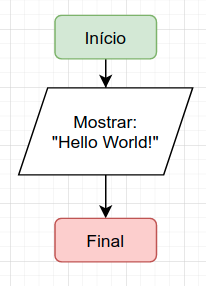
\includegraphics[width=0.25\textwidth]{Pictures/cap01/programa11}
	\caption{Fluxograma do Programa \textbf{Hello World}}
\end{figure}

Salvamos este como hello.asm. Agora em um terminal e digitamos o seguinte comando para compilar o programa: \\
{\ttfamily\$ nasm -f elf64 hello.asm}

Uma vez executado sem erros, o seguinte comando para linkeditar o programa: \\
{\ttfamily\$ ld -s -o hello hello.o}

E podemos executá-lo com o seguinte comando: \\
{\ttfamily\$ ./hello}

E aparece a mensagem: \textbf{Hello World!} no nosso terminal.

\subsection{Magia Negra}\index{Conceitos Introdutórios}

Sei o que vai dizer: "Está bem parecido a algo relacionado com magia negra", mas compreenda que criamos esse programa apenas para saber que tudo está funcionando corretamente e olhe o fluxo dele verá que é algo bem simples. O problema é que as pessoas se preocupam demais em querer aprender tudo em uma simples frase ou mesmo em um único início de seção. Peço apenas que relaxemos pois ainda estamos arranhando a superfície. Temos muito mais coisa para vermos.

Vamos fazer um acordo se ao término dessa seção não compreender o que fizemos, aí sim pode chorar, reclamar e inclusive parar de ler esse livro. Tirando isso, permitamos ter paciência no nosso coração.

\subsection{Explicação do Programa}\index{Conceitos Introdutórios}

Vamos começar entendendo a estrutura do programa. Se divide em 2 partes, uma seção ".data" que é aonde declaramos nossas constantes que utilizaremos ao longo do programa e uma seção ".text" que teremos realmente o que este programa executará. Um marcador em particular deve ser o primeiro e definido através do comando "global" e padronizado com o nome "\_start". Sendo assim a estrutura deve ser essa:
\begin{lstlisting}[]
section .data
	
section .text
	
global _start
	
_start:
\end{lstlisting}

Porém se tentar executar isso verá que teremos um erro, muito comum chamado "\textit{Exec format error}", ou seja, o Sistema Operacional está nos comunicando que não existe nada aí para fazer, e precisamos de um conjunto mínimo de ações para que possa executar sem apresentar qualquer falha. Este mínimo é obtido com as 3 últimas linhas do nosso programa:
\begin{lstlisting}[]
section .data

section .text

global _start

_start:
  mov eax, 0x1
  mov ebx, 0x0
  int 0x80
\end{lstlisting}

E agora não apresenta mais erro, e nenhuma informação. Mas o que essas linhas querem dizer? Assembly trabalha com registradores de memória e isso corresponde a uma tabela que sempre devemos ter em mente quando programamos com esta linguagem:
\begin{table}[H]
	\centering 
	\begin{tabular}{c | c | l }
		\textbf{64 bits} & \textbf{32 bits} & \textbf{Utilização} \\ \hline
		rax & eax & Valores que são retornados dos comandos em um registrador \\
		rbx & ebx & Registrador preservado. Cuidado ao utilizá-lo \\
		rcx & ecx & Uso livre como por exemplo contador \\
		rdx & edx & Uso livre em alguns comandos \\
		rsp & esp & Ponteiro de uma pilha \\
		rbp & ebp & Registrador preservado. Algumas vezes armazena ponteiros de pilhas \\
		rdi & edi & Na passagem de argumentos, contém a quantidade desses \\
		rsi & esi & Na passagem de argumentos, contém os argumentos em si \\
	\end{tabular}
\end{table}

Além desses, existem os registradores de \textbf{r8} a \textbf{r15} (de 64 bits) e \textbf{r8d} a \textbf{r15d} (de 32 bits) que são utilizados nas movimentações correntes durante a nossa programação.

Show demais e isso mas na prática? Bem temos que conhecer como age o comando \textbf{MOV}, este transporta valores de um lugar para outro, porém sua ordem é a seguinte: \textbf{mov destino, origem}. Ou seja, o segundo valor é que será transportado para o primeiro (tem pessoas que leem inversamente). Assim o comando: \\
{\ttfamily mov eax, 0x1}

Está na verdade colocando o valor hexadecimal (indicado pelo prefixo "0x") que corresponde ao valor 1 no registrador \textbf{EAX}. Mas o que isso significa? Esse registrador armazena algumas informações destinadas ao Sistema Operacional e devemos "decorar" esses valores, então vamos fazendo isso a medida que formos utilizando.

Para o registrador \textbf{EAX}:
\begin{table}[H]
	\centering 
	\begin{tabular}{c | c | l }
		\textbf{Decimal} & \textbf{Hexadecimal} & \textbf{Utilização} \\ \hline 
		1 & 0x1 & Indica o final de operação, corresponde a \textbf{System.exit}
	\end{tabular}
\end{table}

Ou seja, ao movermos este valor "0x1" queremos dizer que estamos procedendo uma operação de encerramento, sendo que o valor de \textbf{EBX} é meramente informativo: \\
{\ttfamily mov ebx, 0x0}

Como assim "informativo"? Podemos colocar um valor qualquer, usamos o zero como um padrão para indicar que tudo ocorreu bem com o nosso programa. Troque-o para qualquer outro valor e veja que teremos o mesmo resultado. Para que serve então? Para avisar a um outro programa que nos chamou, obviamente o outro deve saber disso.

Por fim mandamos a informação para o sistema operacional com: \\
{\ttfamily int 0x80}

Esse valor hexadecimal corresponde a 128 em decimal e indica ao SO que agora é com ele e que pode realizar as ações sem problemas. Então a programação é feita assim, preparamos tudo e falamos para o SO: Pode executar.

\subsection{Mostrar a mensagem}\index{Conceitos Introdutórios}
Com tudo o que vimos acima apenas expandimos a ideia para mostrar uma mensagem na saída do terminal, porém primeiro precisamos declarar duas constantes que é feito na seção .data, são elas: \\
\begin{lstlisting}[]
section .data
  msg db 'Hello World!', 0xA
  tam equ $- msg
\end{lstlisting}

O que queremos dizer com isso? quereremos dizer que lá vem mais uma tabela para decorarmos:
\begin{table}[H]
	\centering 
	\begin{tabular}{c | c | l | l }
		\textbf{Sigla} & \textbf{Tipo} & \textbf{Significado} & \textbf{Bytes} \\ \hline
		db & Define Byte & alocação de 8 bits & 1 byte\\
		dw & Define Word & alocação de 16 bits & 2 bytes \\
		dd & Define Doubleword & alocação de 32 bits & 4 byte\\
		dq & Define Quadword & alocação de 64 bits & 8 byte \\
		ddq & Define Double Quad & alocação de 128 bits - para inteiros & 10 bytes \\
		dt & Define Ten Bytes & alocação de 128 bits - para decimais & 10 bytes
	\end{tabular}
\end{table}

Então temos uma marcação chamada "msg" com 8 bits de espaço e o valor em hexadecimal 0xA (que corresponde ao 10 decimal), significa: quebra de linha (line feed). A marcação "tam" contém a quantidade de caracteres que se encontra em "msg", isso é realizado pelo comando "\textit{\$- variável}". A palavra chave "\textbf{equ}" está apenas firmando e declarando que "tam" é uma constante.

Agora a segunda parte no qual fazemos os movimentos e dizemos para o SO, todo seu:
\begin{lstlisting}[]
  mov eax, 4
  mov ebx, 1
  mov ecx, msg
  mov edx, tam
  int 0x80
\end{lstlisting}

Mais dois valores para decorarmos com o registrador \textbf{EAX}:
\begin{table}[H]
	\centering 
	\begin{tabular}{c | c | l }
		\textbf{Decimal} & \textbf{Hexadecimal} & \textbf{Utilização} \\ \hline
		3 & 0x3 & Para operações de leitura, corresponde a \textbf{read} \\
		4 & 0x4 & Para operações de saída, corresponde a \textbf{write}
	\end{tabular}
\end{table}

Agora o registrador \textbf{EBX} passa a ganhar importância e deve receber valores correspondentes a:
\begin{table}[H]
	\centering 
	\begin{tabular}{c | c | l }
		\textbf{Decimal} & \textbf{Hexadecimal} & \textbf{Utilização} \\ \hline
		0 & 0x0 & Indica uma entrada de valor na padrão do Sistema, corresponde a \textbf{System.in} \\
		1 & 0x1 & Indica uma saída de valor na padrão do Sistema, corresponde a \textbf{System.out} \\
	\end{tabular}
\end{table}

Os movimentos realizados nesse registrador são extremamente importantes, ao enviarmos o valor 0x4 significa que realizaremos uma saída de informação, e acompanhando o registrador \textbf{EBX} indica aonde isso será feita, e ele disse 0x1, ou seja, na saída padrão (ou no caso o terminal). O próximo registrador \textbf{ECX} contém o conteúdo em caractere do que desejamos mostrar e por fim o registrador \textbf{EDX} com a quantidade de caracteres que será mostrada (precisa disso? Assembly EXIGE isso).

E assim obtemos nossa mensagem "Hello World!" no terminal.

\subsection{Faltou um comando}\index{Conceitos Introdutórios}

Tá certo sei que faltou: \\
{\ttfamily saida:}

Mas esse não é apenas um marcador (label) que criamos para indicar o início de um bloco, não existe qualquer motivo para ele apenas como uma característica de clareza no código.

E falando em clareza, podemos nos utilizar de comentários. Em Assembly NASM tudo o que estiver depois do ";" será desprezado pelo compilador, sendo extremamente normal as pessoas programarem e colocarem este no final de cada linha, exatamente para indicar o que está fazendo:
\begin{lstlisting}[]
; hello.asm
; programa para mostrar uma mensagem Hello World!
;

; Secao de variaveis
section .data
	msg db 'Hello World!', 0xA ; Mensagem a mostrar
	tam equ $- msg             ; Quantidade de caracteres da mensagem
	
; Secao do Programa	
section .text
	
global _start
	
; Marcador inicial	
_start:
	mov eax, 4    ; Informa que se trata de uma saida
	mov ebx, 1    ; Indica que deve ser realizada no terminal
	mov ecx, msg  ; Conteudo da saida
	mov edx, tam  ; Quantidade de caracteres
	int 0x80      ; Envia a informacao ao Sistema Operacional
	
saida:
	mov eax, 1    ; Informa que terminamos as acoes
	mov ebx, 0    ; Informa o estado final do programa - 0 sem erro
	int 0x80      ; Envia a informacao ao Sistema Operacional
\end{lstlisting}
 
E apesar de ter bem mais informações (poluição visual), fica bem mais claro escrito dessa forma. Então tente tornar isso um hábito quando for escrever seus programas em Assembly.

\section{Programa 1.2 - Entrada}\index{Conceitos Introdutórios}
Outra boa prática que podemos realizar quando se programa com Assembly é colocar todos os dados, que vimos nas tabelas como descritivos de valores. Porém devemos compreender que quando programamos em Assembly temos uma paixão por hexadecimais e normalmente colocamos tudo nessa base.

Nosso programa pode ser descrito conforme o seguinte fluxograma:
\begin{figure}[H]
	\centering
	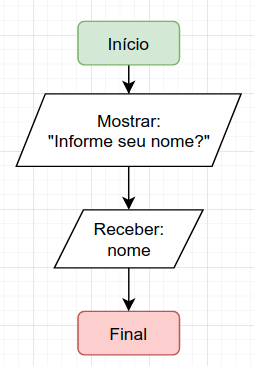
\includegraphics[width=0.25\textwidth]{Pictures/cap01/programa12}
	\caption{Fluxograma do Programa \textbf{Entrada}}
\end{figure}

Ao invés de mostrar o programa inteiro, como fizemos (e provavelmente complexei um monte de leitores) veremos parte a parte deste e assim o montaremos até o resultado final (ou seja iremos assemblando\footnote{Pode parecer meio esquisito isso mas saiba que muitas pessoas usavam a palavra Assemblar como verbo sinônimo para montar - afinal esse é o significado da palavra, até que o termo caiu em desuso.} o programa).

Iniciamos nossa implementação com a adição de um segmento de dado denominado "segment .data", criamos um novo programa chamado "entrada.asm" e digitamos a seguinte informação:
\begin{lstlisting}[]
; entrada.asm	
; Programa para Entrada de Dados
;
segment .data
	LF        equ 0xA  ; Line Feed
	NULL      equ 0xD  ; Final da String
	SYS_EXIT  equ 0x1  ; Codigo de chamada para finalizar
	RET_EXIT  equ 0x0  ; Operacao com Sucesso
	STD_IN    equ 0x0  ; Entrada padrao
	STD_OUT   equ 0x1  ; Saida padrao
	SYS_READ  equ 0x3  ; Operacao de Leitura
	SYS_WRITE equ 0x4  ; Operacao de Escrita
	SYS_CALL  equ 0x80 ; Envia informacao ao SO
\end{lstlisting}

Colocamos todos os valores que já vimos anteriormente em uma tabela associativa de variáveis, assim quando precisamos de algum deles basta chamar pelo nome desta. Mas tem valores repetidos como por exemplo SYS\_EXIT e STD\_OUT porquê não deixar um só? Pois a intenção é mapear os valores e não confundir quando formos escrever o comando, não existe o menor motivo de não gastar variáveis a mais para deixarmos o código mais simples e bem escrito.

Próxima parte e iniciarmos nosso programa com a declaração das variáveis que iremos utilizar e aprendermos uma nova seção:
\begin{lstlisting}[]
section .data
	msg db "Entre com seu nome: ", LF, NULL
	tam equ $- msg

section .bss
	nome resb 1

section .text

global _start

_start:
\end{lstlisting}

Já vimos o que significa a seção .data, porém qual sua diferença para .bss? Essa seção é uma abreviatura de \textit{Block Starting Symbol} e nela colocamos todas as variáveis que serão modificadas pelo programa. Para definir seus valores podemos usar mais uma tabela:
\begin{table}[H]
	\centering 
	\begin{tabular}{c | c | l }
		\textbf{Sigla} & \textbf{Tipo} & \textbf{Significado} \\ \hline
		resb & byte & variável de 8 bits \\
		resw & word & variável de 16 bits \\
		resd & double & variável de 32 bits \\
		resq & quad & variável de 64 bits \\
		resdq & double quad & variável de 128 bits
	\end{tabular}
\end{table}

O comando da seção .bss é bem diferente da seção .data, nessa segunda por exemplo fazemos: \\
{\ttfamily bVar db 10}

E isso significa que criamos uma variável chamada \textbf{bVar} com o valor 10 nela e esse valor foi armazenado em uma variável de 8 bits. Porém se definirmos em .bss: \\
{\ttfamily bVar resb 10}

Estamos agora com um \textit{array} de bytes contendo 10 elementos, repare que é uma diferença bem gritante. Por isso dizemos que em .data colocamos as constantes (mas na verdade também são expressões variáveis), pois lá recebem valores iniciais enquanto que .bss temos as variáveis (e na verdade são arrays de elementos).

Então conforme explicamos e com o auxílio da nossa tabela, criamos uma variável chamada "nome" que contém 1 elemento como array de bytes, que será utilizada para armazenar o valor que informaremos. O próximo bloco mostra ao usuário que ele deve informar um nome:
\begin{lstlisting}[]
	mov eax, SYS_WRITE
	mov ebx, STD_OUT
	mov ecx, msg
	mov edx, tam
	int SYS_CALL
\end{lstlisting}

Ao utilizarmos as variáveis que criamos no segmento, observe que a sintaxe do programa começa a ficar um pouco mais clara, "msg" e "tam" foram definidos na seção .data e contém respectivamente a frase que desejamos mostrar e o tamanho desta.

\subsection{Entrada do nome}\index{Conceitos Introdutórios}

Próximo bloco corresponde a entrada da informação propriamente dita:
\begin{lstlisting}[]
	mov eax, SYS_READ
	mov ebx, STD_IN
	mov ecx, nome
	mov edx, 0xA
	int SYS_CALL
\end{lstlisting}

Os movimentos dos registradores são exatamente os mesmos porém temos uma passagem diferente dos valores das informações, e aí que está toda graça de Assembly pois vemos que transações de entradas e saídas são as mesmas. Para o registrador \textbf{EAX} temos o valor correspondente a uma operação de leitura ao invés de uma escrita. Para o registrador \textbf{EBX} temos o valor correspondente a uma entrada padrão (teclado) ao invés de uma saída padrão (monitor). Os registradores \textbf{ECX} e \textbf{EDX} permanecem com as mesmas informações variável (a diferença que agora o valor informado será armazenado na variável ao invés de obtermos seu conteúdo) e o tamanho.

E esta último preenchimento torna-se um problema, isso limita a entrada do usuário, nesse caso usamos o hexadecimal 0xA que corresponde ao decimal 10, assim sendo o usuário só pode colocar um nome contendo 10 caracteres, se ultrapassar esse valor a informação será cortada. Em breve resolveremos isso, mas por enquanto deixaremos como está.

A última parte do programa também já vimos:
\begin{lstlisting}[]
	mov eax, SYS_EXIT
	mov ebx, RET_EXIT
	int SYS_CALL
\end{lstlisting}

Que avisa ao sistema operacional que encerramos todas as atividades e agora pode encerrar os usos desse programa limpando as áreas de memória ou outras alocações realizadas por ele.

\subsection{Compilação e Linkedição}\index{Conceitos Introdutórios}

Ao invés de ficarmos sofrendo tendo que inserir 2 comandos (até parece que é muita coisa) para compilar e linkeditar nosso programa, vamos criar um arquivo especial que realiza esse trabalho. Obrigatoriamente seu nome deve ser \textbf{makefile}, então crie um arquivo com esse nome e digite os seguintes comandos:
\begin{lstlisting}[]
NOME = entrada

all: $(NOME).o
	ld -s -o $(NOME) $(NOME).o
	rm -rf *.o;

%.o: %.asm
	nasm -f elf64 $<
\end{lstlisting}

Pode parecer bem estranho mas este programa faz exatamente o que esses três comandos fariam: \\
{\ttfamily\$ nasm -f elf64 entrada.asm} \\
{\ttfamily\$ ld -s -o entrada entrada.o} \\
{\ttfamily\$ rm entrada.o}

No início criamos uma variável \textbf{NOME} facilitando assim sua modificação nos próximos programas pois basta modificar essa variável para o nome do programa atual e tudo está pronto. Para executar esse programa digite o seguinte: \\
{\ttfamily\$ make}

Não erramos na digitação é assim mesmo, disse que era um arquivo especial. E pronto, uma vez executado corretamente o programa sera compilado e linkeditado. Ao executá-lo com: \\
{\ttfamily\$ ./entrada}

Será mostrado: \\
{\ttfamily\$ Entre com seu nome:}

E o cursor espera que seja informado algo e pressionado a tecla ENTER para dar continuidade ao programa.

\section{Programa 1.3 - Comparar Valores}\index{Conceitos Introdutórios}
Neste programa vamos realizar comparações entre valores e compreender como saltos condicionais e incondicionais funcionam na linguagem. Assembly realiza comparações com 2 comandos, um deles normalmente é o comando \textbf{CMP} (outros fazem esse mesmo serviço) que possui a sintaxe: \\
{\ttfamily\$ cmp registrador1, registrador2}

E aí pergunta-se: está comparando os registradores como? Aí entra um segundo comando que executará o salto para determinado ponto do programa, vamos para mais uma tabela:
\begin{table}[H]
	\centering 
	\begin{tabular}{c | l | c | l }
		\textbf{Mnemônico} & \textbf{Significado} & \textbf{Contrário} & \textbf{Significado} \\ \hline
		JE & Salta se igual & JNE & Salta se não igual \\
		JG & Salta se maior & JNG & Salta se não maior \\
		JL & Salta se menor & JNL & Salta se não menor \\
		JGE & Salta se maior ou igual & JNGE & Salta se não maior ou igual \\
		JLE & Salta se menor ou igual & JNLE & Salta se não menor ou igual \\
	\end{tabular}
\end{table}

Esses saltos são chamados de "condicionais", ou seja, dependem que uma comparação ocorra. Porém ainda existe o comando \textbf{JMP} que é um salto "incondicional", isso é, não depende que nada ocorra. E posto tudo isso o nosso programa deveria ter a aparência conforme o primeiro fluxograma (e assim ficaria em linguagens de alto nível), porém no Assembly nosso programa terá a aparência do segundo:
\begin{figure}[ht]
	\begin{minipage}[b]{0.45\linewidth}
		\centering
		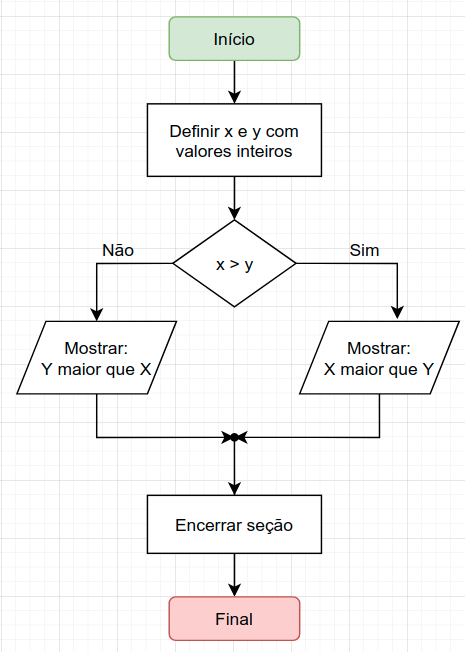
\includegraphics[width=0.80\textwidth]{Pictures/cap01/programa13a}
		\caption{Fluxograma estruturado}
	\end{minipage}
	\hspace{0.5cm}
	\begin{minipage}[b]{0.45\linewidth}
		\centering
		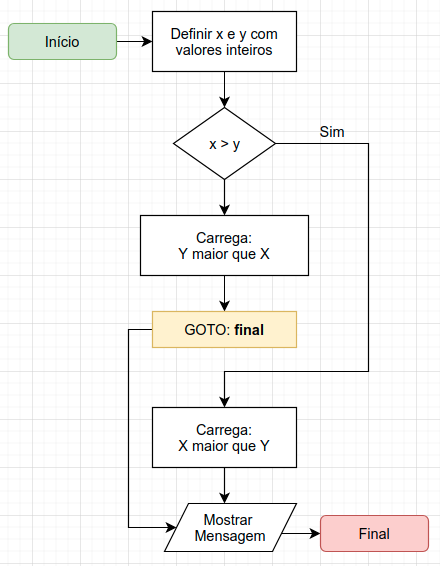
\includegraphics[width=0.85\textwidth]{Pictures/cap01/programa13}
		\caption{Do programa \textbf{Comparar Valores}}
	\end{minipage}
\end{figure}

Mas qual o motivo dessa diferença tão gritante? Assembly não possui um comando interno que toma uma decisão e faz blocos de desvios, os blocos de desvio do Assembly são simplesmente pontos "etiquetados" do nosso programa. Lembra no início que criamos um "\_start:", pois bem isso não é uma função (como seria em linguagens de alto nível) isso é um \textit{label} (ou um MARCADOR se prefere a palavra em português que é a palavra que usamos neste livro).

Vamos iniciar um programa chamado maiornum.asm, copiamos o nosso segmento de dados (os mesmos vistos anteriormente) e criamos as seguintes variáveis na seção \textbf{.data}:
\begin{lstlisting}[]
segment .data
	LF        equ 0xA  ; Line Feed
	NULL      equ 0xD  ; Final da String
	SYS_EXIT  equ 0x1  ; Codigo de chamada para finalizar
	RET_EXIT  equ 0x0  ; Operacao com Sucesso
	STD_IN    equ 0x0  ; Entrada padrao
	STD_OUT   equ 0x1  ; Saida padrao
	SYS_READ  equ 0x3  ; Operacao de Leitura
	SYS_WRITE equ 0x4  ; Operacao de Escrita
	SYS_CALL  equ 0x80 ; Envia informacao ao SO

section .data
	x dd 10
	y dd 50
	msg1 db 'X maior que Y', LF, NULL
	tam1 equ $ - msg1
	msg2 db 'Y maior que X', LF, NULL
	tam2 equ $ - msg2
\end{lstlisting}

Temos duas variáveis a primeira chamada \textbf{x} que possui o valor de 10 e a segunda \textbf{y} com o valor de 50, ao término altere esses valores para testar completamente o programa. Temos também \textbf{msg1} que mostra "X maior que Y" e \textbf{msg2} para mostrar o inverso, ou "Y maior que X" além de \textbf{tam1} e \textbf{tam2} para armazenar o tamanho das mensagens respectivamente. Agora vamos começar nosso programa propriamente dito pela seção \textbf{.text}:

\begin{lstlisting}[]
section .text

global _start

_start:
	mov eax, DWORD [x]
	mov ebx, DWORD [y]
\end{lstlisting}

Iniciamos com 2 movimentos de \textbf{x} e \textbf{y} para os registradores \textbf{EAX} e \textbf{EBX} fazendo uma conversão relativa para \textbf{DWORD}. Não é possível mover o conteúdo de um DD diretamente para estes registradores.

\begin{lstlisting}[]
	cmp eax, ebx
	jge maior
\end{lstlisting}

Em seguida procedemos a comparação entre os dois registradores e perguntamos se o registrador \textbf{EAX} (o primeiro) é maior ou igual (\textbf{JGE}) que \textbf{EBX} (o segundo), caso seja salta para uma etiqueta chamada \textbf{maior}. Caso não seja maior ou igual o programa continuará em seu fluxo normal.

\begin{lstlisting}[]
	mov ecx, msg2
	mov edx, tam2
	jmp final
\end{lstlisting}

No fluxo normal colocamos a \textbf{msg2} no registrador \textbf{ECX} e seu tamanho em \textbf{EDX}, e fazemos um salto incondicional para uma etiqueta chamada \textbf{final}.

\begin{lstlisting}[]
maior:
	mov ecx, msg1
	mov edx, tam1
\end{lstlisting}

Declaramos a etiqueta \textbf{maior} e colocamos a \textbf{msg1} no registrador ECX e seu tamanho em EDX.

\begin{lstlisting}[]
final:
	mov eax, SYS_WRITE
	mov ebx, STD_OUT
	int SYS_CALL
\end{lstlisting}

Declaramos a etiqueta \textbf{final}, sendo aqui que os dois pontos do programa se encontram. Fazemos os dois movimentos finais para mostrar o resultado, como já carregamos \textbf{ECX} e \textbf{EDX} anteriormente a mensagem será mostrada de forma correta.

\begin{lstlisting}[]
	mov eax, SYS_EXIT
	mov ebx, RET_EXIT
	int SYS_CALL 
\end{lstlisting}

E fazemos o movimento final encerrando a seção. Pronto agora podemos executar (compilar e linkeditar com uma cópia do arquivo MAKEFILE visto anteriormente, modificar valor da variável NOME) e testar vários valores para X e Y.

\section{Programa 1.4 - Converter}\index{Conceitos Introdutórios}
Antes mesmo de começarmos nosso programa, vamos criar uma biblioteca e assim parar de copiar os códigos da "segment .data", além de começarmos a criar alguns marcadores globais que podemos usar de uma forma mais consistente.

Para criar uma biblioteca, crie um novo arquivo com o nome "bibliotecaE.inc" e neste insira a seguinte codificação:
\begin{lstlisting}[]
segment .data
	LF        equ 0xA  ; Line Feed
	NULL      equ 0xD  ; Final da String
	SYS_EXIT  equ 0x1  ; Codigo de chamada para finalizar
	RET_EXIT  equ 0x0  ; Operacao com Sucesso
	STD_IN    equ 0x0  ; Entrada padrao
	STD_OUT   equ 0x1  ; Saida padrao
	SYS_READ  equ 0x3  ; Operacao de Leitura
	SYS_WRITE equ 0x4  ; Operacao de Escrita
	SYS_CALL  equ 0x80 ; Envia informacao ao SO

  	TAM_BUFFER equ 0xA

segment .bss
	BUFFER resb 0x1
\end{lstlisting}

Agora para o nosso programa que chamaremos de "converte.asm" na primeira linha insira o seguinte código:
\begin{lstlisting}[]
%include 'bibliotecaE.inc'
\end{lstlisting}

A definição de \textbf{TAM\_BUFFER} e \textbf{BUFFER} veremos nos marcadores propostos, por enquanto só necessitamos saber que a segunda é um binário que carrega um determinado valor a ser utilizado.

E estamos prontos, daqui para frente salvo qualquer outra observação sempre que criarmos um programa o primeiro passo será copiar o conteúdo da "bibliotecaE.inc" e adicionar a cláusula \textbf{\%include}. Além obviamente do arquivo "Makefile" para compilarmos e linkeditarmos o programa. Sempre partirei (para não me tornar repetitivo) do princípio que essas ações já aconteceram.

Vamos começar adicionando um simples marcador, que já vimos ser executado várias vezes, e deve ser adicionada na "bibliotecaE.inc":

\begin{lstlisting}[]
segment .text

; ---------------------------------------------
; Saida do Resultado no Terminal
; ---------------------------------------------
; Entrada: valor String em BUFFER
; Saida: valor no terminal
; ---------------------------------------------
saidaResultado:
	mov eax, SYS_WRITE
	mov ebx, STD_OUT
	mov ecx, BUFFER
	mov edx, TAM_BUFFER
	int SYS_CALL
	ret
\end{lstlisting}

Marcadores são criadas na biblioteca para nossa comodidade, acho que o único detalhe que ainda precisamos entender é esse comando \textbf{ret}, pois para o resto basta olhar desde o primeiro programa que construímos para entender seu funcionamento. Quando saltos são dados (sejam eles condicionais ou incondicionais) não existe um retorno ao ponto de partida, ao chamarmos um marcador é diferente esperamos que retornem, é exatamente isso que faz o comando \textbf{RET}, desvia o fluxo de volta para a próxima instrução onde este marcador foi chamado (ou seja por um comando \textbf{CALL}).

\subsection{Criar o nosso programa}\index{Conceitos Introdutórios}
Neste programa vamos compreender 2 ações muito comuns que acontece em programação a conversão de uma cadeia de caracteres para um número e vice versa. Observe seu fluxograma:
\begin{figure}[H]
	\centering
	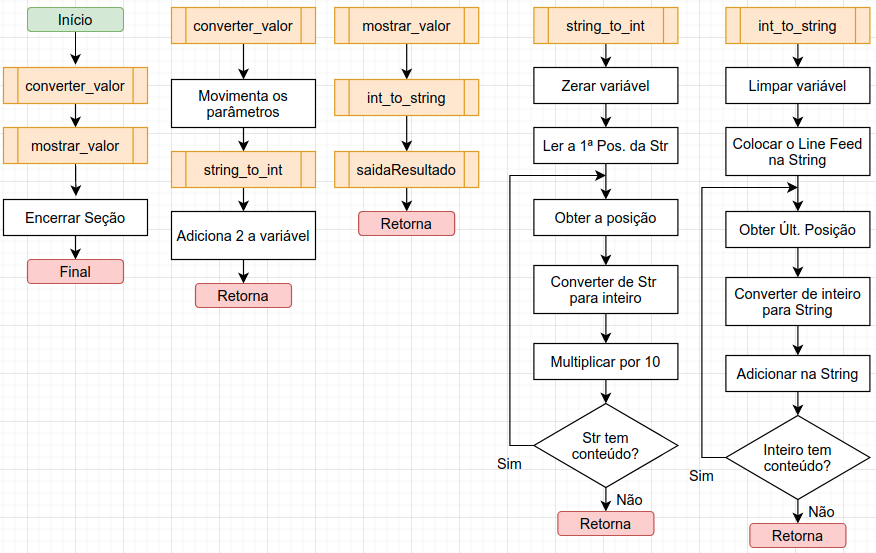
\includegraphics[width=0.65\textwidth]{Pictures/cap01/programa14}
	\caption{Fluxograma do Programa \textbf{Converter}}
\end{figure}

Uma característica bem curiosa que o programa será completamente "modular" ou seja, será dividido em pequenos blocos. Vamos começar a montagem inicial:
\begin{lstlisting}[]
section .data
	v1 dw '105', 0xa

section .text
global _start

_start:
	call converter_valor
	call mostrar_valor
	mov eax, SYS_EXIT
	mov ebx, RET_EXIT
	int SYS_CALL
\end{lstlisting}

Na seção \textbf{.data} criamos o valor que iremos converter em uma variável chamada \textbf{v1} do tipo Double Word (ou seja um caracter). Já quando começamos o programa em si temos 2 comandos \textbf{CALL}, que no fluxograma corresponde as duas primeiras caixas laranjas, este comando é responsável por chamar um ponto do programa (marcado), aguardar seu retorno e continuar a partir desse ponto. E encerramos a nossa seção do programa, ou seja, podemos dizer que o principal é só isso, e observe realmente que pelo fluxo está totalmente correto.
\begin{lstlisting}[]
converter_valor:
	lea esi, [v1]
	mov ecx, 0x3
	call string_to_int
	add eax, 0x2
	ret
\end{lstlisting}

O próximo módulo é responsável por transpor o valor de \textbf{v1} para o registrador \textbf{ESI} e seu tamanho para \textbf{ECX}, em seguida chamar o marcador \textbf{string\_to\_int} para realizar a conversão dessa variável em inteiro. O valor de convertido estará contido no registrador \textbf{EAX} e a ele adicionaremos mais 2 (apenas para testar se realmente virou inteiro) e retornamos ao ponto que chamou.

O comando \textbf{LEA} permite que calculemos efetivamente o endereço de qualquer elemento em uma tabela (ou um endereço) e elimina este endereço em um registrador. Ou seja, diferente do comando \textbf{MOV} é um caminho mais seguro em se tratando de movimentações de variáveis para registradores.

\begin{lstlisting}[]
mostrar_valor:
	call int_to_string
	call saidaResultado
	ret
\end{lstlisting}

Este trecho chama o marcador \textbf{int\_to\_string} para realizar a conversão da variável (que deve estar no registrador EAX) de volta para uma cadeia de caracteres como forma a dar saída no terminal através do marcador (contida em nossa biblioteca) "saidaResultado".

Agora podemos escolher se colocaremos esses dois trechos no programa ou na biblioteca, recomendamos sempre que criar uma novo trecho marcado coloque-o primeiro no programa e teste-o, caso tudo funcione corretamente transfira-o para a biblioteca. Porém as bibliotecas que usaremos não devem conter sujeira (códigos não utilizáveis pelo programa) pois senão geraríamos apenas lixo e aumento do tamanho desnecessário no nosso executável final. Ou seja, mantenha esses trechos de código a mão quando necessários o seu uso, mas não os coloque sempre para QUALQUER programa que crie.

\subsection{Realização de Conversão}\index{Conceitos Introdutórios}

Antes de começarmos a ver as conversões devemos entender que os operadores: AH, AL, BH, BL, CH, CL, DH e DL são o que chamamos de segmentos de 8 bits. Toda vez que tratamos de um único caractere temos um byte isolado (ou seja 8 bits) e podemos usar esses operadores para realizar algumas transformações como veremos a seguir.

Convertendo da cadeia de caracteres para inteiro:
\begin{lstlisting}[]
string_to_int:
	xor ebx, ebx

.prox_digito:
	movzx eax, byte[esi]
	inc esi
	sub al, '0'
	imul ebx, 0xA
	add ebx, eax
	loop .prox_digito
	mov eax, ebx
	ret
\end{lstlisting}

Este trecho espera que o registrador \textbf{ESI} contenha o valor a ser convertido e \textbf{ECX} a quantidade de caracteres deste. O primeiro passo é zerar o registrado \textbf{EBX}, o comando \textbf{XOR} é um comparador de bit no qual se ambos forem iguais (isto é, ambos 0 ou 1) o resultado será 0 para aquela posição de bit, isso é uma forma elegante de dizer que algo recebe 0 ao invés de simplesmente enviar 0x0.

O comando \textbf{MOVZX} é abreviatura para \textit{Move with Zero-Extend}, isso significa que os bits superiores do operador de destino serão preenchidos com zero. Próximo passo é incrementar a posição do registrador \textbf{ESI} e achar o valor correspondente da letra. A instrução "\textit{sub al,'0'}" converte o caractere em \textbf{AL} isso corresponde a um número entre 0 e 9.

Agora multiplicamos o registrador \textbf{EBX} por 10 e adicionamos o conteúdo de \textbf{EAX} a este. O comando \textbf{LOOP} salta para pegar o próximo registro e assim será realizado até que todos os caracteres da cadeia tenha sido lidos. Ao término movemos o conteúdo de \textbf{EBX} para \textbf{EAX} de modo a retornar o valor.

Vamos na prática, nosso valor é "105", então o primeiro caractere é "1" e será convertido para inteiro, EBX inicial vale 0 que será multiplicado por 10 resultando 0 e assim EBX terá o valor 1. Na próxima interação vem o caractere "0" que é convertido e EBX que contém 1 multiplicado por 10, adicionado a 0 permanece 10. Na última interação o caractere "5" que é convertido e EBX que contém 10 é multiplicado por 10, adicionado a 5 o resultado é 105. Ou seja, o mesmo valor da cadeia de caracteres.

Convertendo da cadeia de caracteres para inteiro:
\begin{lstlisting}[]
int_to_string:
	lea esi, [BUFFER]
	add esi, 0x9
	mov byte[esi], 0xA
	mov ebx, 0xA

.prox_digito:
	xor edx, edx
	div ebx
	add dl, '0'
	dec esi
	mov [esi], dl
	test eax, eax
	jnz .prox_digito
	ret
\end{lstlisting}

Este trecho espera que um valor inteiro esteja armazenado no registrador \textbf{EAX}, o primeiro passo é associar o conteúdo de BUFFER ao registrador \textbf{ESI}, ou seja, tudo o que fizermos com este será refletido para o conteúdo de buffer. Adicionamos o valor 9 a \textbf{ESI} e o movemos 10 para a posição final deste (isso é realizado para que a cadeia possa conter o Line Feed), iniciamos \textbf{EBX} com o valor 10.

No marcador de repetição zeramos \textbf{EDX} e realizamos uma divisão entre \textbf{EBX} e \textbf{EDX}, a instrução "\textit{add dl,'0'}", transforma o valor correspondente ao caractere na tabela ASCII. Agora decrementamos 1 posição de \textbf{ESI} e adicionamos esse valor convertido. Próximo passo é testar (comando \textbf{TEST}) o registrador \textbf{EAX} para saber se ainda existem valores a serem adicionados, se sim salta de volta para obter esse próximo registro caso contrário retorna para a posição de quem chamou este marcador.

Na prática, nosso valor será 107, começamos montando a cadeia com um "LF", e pegamos o primeiro elemento que é o valor 7, convertemos este e adicionamos na cadeia que agora será "7LF", no próximo passo o valor 0 é obtido que resulta em "07LF", e por fim, o valor 1 resultando na cadeia final "107LF".

Mas qual o sentido da divisão? Note que quando convertemos da cadeia para inteiro fomos percorrendo caractere a caractere pois podemos fazer isso em uma cadeia, porém em um número isso é impossível ir de frente para trás, então temos que andar de trás para frente.

Pronto já podemos compilar, linkeditar e executar o programa. Lembre-se que se for testar com valores diferentes de 3 casas modificar o registrador ECX, na instrução "\textit{mov ecx,0x3}", para refletir esta mudança. Além disso qualquer valor colocado será aumentado em 2 conforme a instrução "\textit{add eax,0x2}".

\section{Programa 1.5 - Calculadora}\index{Conceitos Introdutórios}
Como último programa para fecharmos esse capítulo vamos construir o menu completo para uma calculadora que realiza as quatro operações básicas. Na primeira parte solicita 2 valores e em seguida qual operação deve realizar adicionar, subtrair, multiplicar ou dividir. Porém não fique triste pois não iremos realizar as operações apenas mostrar uma saída informando que chegamos ao ponto correto.

Para realizar cada uma das operações seriam necessárias muitas movimentações, mas prometo que em breve faremos isso, por enquanto precisamos apenas fixar esses conhecimentos básicos e o uso dos registrados "E" (de 32 bits) para podermos seguir adiante.

\subsection{Novas funcionalidades a biblioteca}\index{Conceitos Introdutórios}
Observe que um menu existem muitas saídas de dados, e isso é uma característica preocupante pois temos que repetir várias vezes os mesmos comandos, além de criar aquela variável que guarda o tamanho da cadeia de caracteres. Então vamos resolver esses dois problemas primeiro e adicionar dois novos marcadores principais na nossa biblioteca.

\begin{lstlisting}[]
; ---------------------------------------------
; Calcular o tamanho da String
; ---------------------------------------------
; Entrada: valor String em ECX
; Saida: tamanho da String em EDX
; ---------------------------------------------
tamStr:  
	mov edx, ecx
proxchar:
	cmp byte[edx], NULL
	jz terminei
	inc edx
	jmp proxchar  
terminei:
	sub edx, ecx
	ret
\end{lstlisting}

Vamos passar uma cadeia de caracteres no registrador \textbf{ECX} e de modo bem simples vamos contar (tem que ser manualmente pois não existe um comando que realize isso) caractere a caractere, observe que no inicio mantemos o valor de \textbf{ECX} em \textbf{EDX}, o conteúdo do centro é simples conta todos os caracteres até achar o valor NULL (0xD). O pulo do gato está no comando \textbf{SUB} (que possui a sintaxe \textit{sub destino, secundário}). Isso parace bem esquisito para quem vem das linguagens de alto nível: \textbf{EDX} contém 2 valores, o primeiro é a cadeia de caracteres e o segundo um valor inteiro contendo os incrementos que fizemos no centro, se queremos somente o valor inteiro basta remover essa cadeia de caracteres (para isso subtraímos).

\begin{lstlisting}[]
; ---------------------------------------------
; Saida do Resultado no Terminal
; ---------------------------------------------
; Entrada: String em ECX
; Saida: valor no terminal
; ---------------------------------------------
mst_saida:
	call tamStr
	mov eax, SYS_WRITE
	mov ebx, STD_OUT
	int SYS_CALL
	ret
\end{lstlisting}

Para nosso marcador de saída, recebemos a cadeia de caractere através do registrador \textbf{ECX}, chamamos o marcador descrito anteriormente para obtermos tamanho que virá em \textbf{EDX}. Agora basta finalizar com os valores de \textbf{EAX}, \textbf{EBX} e informar ao sistema operacional que pode processar.

\subsection{Menu de Sistema}\index{Conceitos Introdutórios}

Nosso processo começa com a declaração de todas as variáveis que utilizaremos ao longo do programa:
\begin{lstlisting}[]
%include 'bibliotecaE.inc'

section .data
	tit     db LF,'+-------------+',LF,'| Calculadora |',LF,'+-------------+', NULL
	obVal1  db LF,'Valor 1:', NULL
	obVal2  db LF,'Valor 2:', NULL
	opc1    db LF,'1. Adicionar', NULL
	opc2    db LF,'2. Subtrair', NULL
	opc3    db LF,'3. Multiplicar', NULL
	opc4    db LF,'4. Dividir', NULL
	msgOpc  db LF,'Deseja Realizar?', NULL
	msgErro db LF,'Valor da Opcao Invalido', NULL
	p1      db LF,'Processo Adicionar', NULL
	p2      db LF,'Processo Subtrair', NULL
	p3      db LF,'Processo Multiplicar', NULL
	p4      db LF,'Processo Dividir', NULL
	msgfim  db LF,'Terminei.', LF, NULL

section .bss
	opc     resb  1
	num1    resb  1
	num2    resb  1
\end{lstlisting}

Um fator importante é que cada cadeia de caracteres deve obrigatoriamente terminar com o caractere NULL, senão nossa marcador de conta calculará totalmente errado. Temos 3 variáveis na seção .bss a opção que o usuário pode escolher e os dois valores para realizar a operação.

\begin{lstlisting}[]
section .text
global _start

_start:
	mov ecx, tit     ; '+-------------+',LF,'| Calculadora |',LF,'+-------------+'
	call mst_saida
\end{lstlisting}

Começamos nossa programação mostrando o título inicial que como resultado deve mostrar no terminal: \\
{\ttfamily +--------------------------+ } \\
{\ttfamily | Calculadora | } \\
{\ttfamily +--------------------------+ }

\begin{lstlisting}[]
	mov ecx, obVal1   ; Valor 1:
	call mst_saida
	mov eax, SYS_READ
	mov ebx, STD_IN
	mov ecx, num1
	mov edx, 0x3
	int SYS_CALL	
\end{lstlisting}

Solicitamos a entrada do primeiro valor para o usuário que mostra a mensagem: "Valor 1:" e fica aguardando. Uma vez informado este irá para a variável \textbf{num1}.

\begin{lstlisting}[]
	mov ecx, obVal2   ; Valor 2:
	call mst_saida
	mov eax, SYS_READ
	mov ebx, STD_IN
	mov ecx, num2
	mov edx, 0x3
	int SYS_CALL
\end{lstlisting}

Processamos de mesma forma agora para solicitar o segundo valor (não valeria a pena criar uma marcador isolado para isso? Utilize como um exercício de formatura desse capítulo).

\begin{lstlisting}[]
	mov ecx, opc1     ; 1. Adicionar
	call mst_saida
	mov ecx, opc2     ; 2. Subtrair
	call mst_saida
	mov ecx, opc3     ; 3. Multiplicar
	call mst_saida
	mov ecx, opc4     ; 4. Dividir
	call mst_saida
\end{lstlisting}

Mostramos agora as quatro opções disponíveis para nosso usuário de modo que possa fazer sua escolha, que resulta em: \\
{\ttfamily 1. Adicionar} \\
{\ttfamily 2. Subtrair} \\
{\ttfamily 3. Multiplicar} \\
{\ttfamily 4. Dividir}

\begin{lstlisting}[]
	mov ecx, msgOpc     ; Deseja Realizar?
	call mst_saida
	mov eax, SYS_READ
	mov ebx, STD_IN
	mov ecx, opc
	mov edx, 2
	int SYS_CALL
\end{lstlisting}

E solicitamos que o usuário determine uma opção (é realmente isso está implorando um marcador isolado, observe que temos exatamente os mesmos comandos porém com valores distintos).

\begin{lstlisting}[]
	mov ah, [opc]
	sub ah, '0'
\end{lstlisting}

Toda entrada é realiza em cadeia de caracteres, se desejamos realizar comparações devemos converter o valor para inteiro, como é um único caractere que será informado basta subtrair por '0' que teremos o valor em inteiro. Como assim? Agora vamos ter que pensar na tabela ASCII, a posição do '0' nesta corresponde ao valor decimal 48 (ou 0x30 se prefere em hexadecimal), os próximos números estão em sequencia, assim '1' corresponde a 49 e assim sucessivamente. Ou seja, se subtraímos o valor 49 (caractere '1') por 48 (caractere '0') temos o decimal 1.

\begin{lstlisting}[]
	cmp ah, 1
	je adicionar
	cmp ah, 2
	je subtrair
	cmp ah, 3
	je multiplicar
	cmp ah, 4
	je dividir
\end{lstlisting}

Agora é realizar os comparativos para saber qual opção nosso usuário selecionou. E se não entrar em nenhuma dessas opções:

\begin{lstlisting}[]
	mov ecx, msgErro  ; Valor da Opcao Invalido
	call mst_saida
	jmp exit
\end{lstlisting}

Mostrar a mensagem de erro para opção inválida e sair do programa.

\begin{lstlisting}[]
adicionar:
	mov ecx, p1       ; Processo Adicionar
	call mst_saida
	jmp exit

subtrair:
	mov ecx, p2       ; Processo Subtrair
	call mst_saida
	jmp exit

multiplicar:
	mov ecx, p3       ; Processo Multiplicar
	call mst_saida
	jmp exit

dividir:
	mov ecx, p4       ; Processo Dividir
	call mst_saida
	jmp exit
\end{lstlisting}

Agora cada marcador será bem similar, apenas modificando a mensagem para termos a certeza que entrou na opção correta. E por fim:
\begin{lstlisting}[]
exit:
	mov ecx, msgfim    ; Terminei.
	call mst_saida

	mov eax, SYS_EXIT
	mov ebx, RET_EXIT
	int SYS_CALL
\end{lstlisting}

Mostrar a mensagem de término e encerrar a seção. 

\section{Programa 1.6 - Arrays}\index{Conceitos Introdutórios}
Vetores (ou Arrays se prefere o termo mais técnico) em Assembly são extremamente comuns, nem sentimos quando estamos o usando, essa frase é tão verdadeira que as pessoas nem reparam que isso aqui em um array:
\begin{lstlisting}[]
	msg1: DB 'Parte 1', LF, NULL
	msg2: DB 'Parte 2', LF, NULL
	msg3: DB 'Parte 3', LF, NULL
	msg4: DB 'Parte 4', LF, NULL
\end{lstlisting}

Pronto peguei um erro nesse livro e esse autor é doido, isso são quatro variáveis! Muitas pessoas agora vão estar pensando isso, mas deixe-me esclarecer, por tudo o que vimos até o momento o que significa qualquer coisa e depois um dois pontos? Isso mesmo um MARCADOR, mas espera aí isso são nomes de var... Não meu gafanhoto isso são marcadores a um determinado ponto do programa. E um detalhe os dois pontos não importam nem são obrigatórios (pode tirá-los e verá que o programa continua mas essa regra não se aplica aos marcadores da seção \textbf{.text}). 

Vamos brincar um pouco a palavra 'Parte 1' + LF + NULL contém 9 caracteres certo, então vamos criar o seguinte programa:
\begin{lstlisting}[]
%include 'bibliotecaE.inc'

SECTION .data
  msg1: DB 'Parte 1', LF, NULL
  msg2: DB 'Parte 2', LF, NULL
  msg3: DB 'Parte 3', LF, NULL
  msg4: DB 'Parte 4', LF, NULL

SECTION .text

global _start

_start:
  mov eax, 4
  mov ebx, 1
  mov ecx, msg1
  mov edx, 36
  int 0x80

  mov eax, 1
  mov ebx, 5
  int 0x80  
\end{lstlisting}

Se cada linha tem 9 caracteres as 4 linhas terão 36 deles por isso \textbf{EDX} contém esse valor (deixei em decimal mesmo para não causar confusão mas se quiser pode usar 0x24). Ao compilar e executar o programa temos: \\
{\ttfamily Parte 1} \\
{\ttfamily Parte 2} \\
{\ttfamily Parte 3} \\
{\ttfamily Parte 4}

Agora façamos 2 mudanças, mover msg3 para \textbf{ECX} e 18 para \textbf{EDX}, e obviamente como resultado temos: \\
{\ttfamily Parte 3} \\
{\ttfamily Parte 4}

É exatamente por esse motivo que usamos o NULL no final para podermos identificar essa posição e aplicarmos um corte quando vimos o marcador \textbf{tamStr} que calcula o tamanho da cadeia de caracteres a mostrar. 

\subsection{Arrays de Inteiros}\index{Conceitos Introdutórios}
Mas como seria um Array de inteiros? No programa \textbf{Converter} temos dois marcadores que utilizaremos aqui, são eles: \textbf{int\_to\_string} e \textbf{saidaResultado}. Adicionamos ambos a nossa biblioteca.

Criar um arquivo chamado "arrays.asm" e vamos iniciá-lo com o seguinte conteúdo:
\begin{lstlisting}[]
%include 'bibliotecaE.inc'

SECTION .data
	array: DD 10, 22, 13, 14, 55
\end{lstlisting}

Definimos um array (não é por causa do nome do marcador - poderíamos ter colocado "casinha" para este) com 5 números, agora devemos pensar o seguinte, cadê a posição de cada um? Temos um DD, isso significa "Define Doubleword" que aloca 4 bytes (a chave aqui é o número de bytes). Então para obtermos qualquer posição precisamos de uma simples equação: \\
{\ttfamily [nome marcador] + 4 * [posição]}

Então se fizermos:
\begin{lstlisting}[]
SECTION .text

global _start:

_start:
  mov eax, [array + 4 * 3]
  call int_to_string
  call saidaResultado

saida:
  mov eax, SYS_EXIT
  mov ebx, EXIT_SUCESS
  int SYS_CALL 	
\end{lstlisting}

Qual será a resposta desse programa? Isso mesmo \textbf{14} que é a nossa \textbf{4º posição}, mas espera foi  colocado 3 e isso não corresponde a 3ª? Não pois a primeira posição é o número 0 e agora acabou de compreender porquê em QUALQUER linguagem de alto nível TODO índice do array começa com 0 e não 1.

Aprender Assembly não vai lhe tornar um Hacker, nem você vai criar sistemas complexos com este. Aprender Assembly faz conhecer detalhes das linguagens que normalmente as pessoas não conhecem e não sabem porquê é feito dessa maneira. E finalizamos esta parte introdutória da linguagem Assembly no próximo capítulo veremos uma junção desta com a linguagem C++.

% Final do Capítulo
\clearpage